\documentclass[12pt,a4]{report}
\usepackage{graphicx}

\begin{document}
\title{%
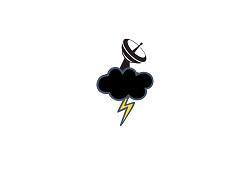
\includegraphics[scale=1.5]{mobicharged.png}~\\
Project MobiCharged: Problem Statement \& Goals}
\author{Nashit Mohammad - mohamn31\\Eric Nguyen - nguyee13\\Samuel De Haan - dehaas1\\Eamon Earl - earle2\\Mustafa Choueib - choueibm}
\date{March 3rd 2023 (R.1)}

\maketitle

\newpage

\begin{center}
\begin{table}
	\caption{\bf Revision History}
	\begin{tabular}{p{2cm}p{3cm}p{2cm}p{6cm}}
		\hline
		\bf Author & \bf Date & \bf Version & \bf Description\\
		\hline
		All & September 24, 2022 & Rev 0 & Created first draft of document\\
		\hline
		Nashit & March 3, 2023 & Rev 1 & Updated title, revision history and applied feedback from Rev 0\\
		\hline
		Nashit & March 3, 2023 & Rev 1 & Replaced "Data Collection" goal with "Continous Data Collection" to accurately reflect updated goals\\
		\hline
		Nashit & March 3, 2023 & Rev 1 & Replaced "Prototype is Resilient to External Environment Conditions" goal with "Prototype is Operational" goal to accurately reflect updated goals\\
		\hline
	\end{tabular}
\end{table}
\end{center}

\clearpage

\section*{Introduction}
The construction industry is not only essential for the ever-growing infrastructure of our society but also a key factor used to determine the success in communities. With the Greater-Toronto-Area being one of the top-rated increasing communities in regards to construction from across the globe, it is salient to ensure any buildings whether residential, commercial or industrial are built with the highest of standard, highlight the importance of safety, and promote on-going innovation.

Engineers are tasked with design in construction to exceed requirements without hindering safety. Safety is a topic that is never missed within the industry and is continuously being highlighted amongst designs; especially as Engineers are reminded of their moral obligations to society by their awarded rings upon graduation. 

As a current process, the construction industry places sensors within concrete spaces to continuously test and/or monitor the integrity of buildings during, as well as after completion of construction. Ultimately however, these sensors run out of battery and are required to be re-charged. The industry still faces challenges when attempting to charge these sensors with the method of remote charging.

There are a significant number of buildings being built in the Greater-Toronto-Area, which is emphasized with the fact that 70\% of cranes within Canada are in just the GTA alone. To place innovation in the sub-field of safety within the industry, it is indeed a requirement to modernize the ability of producing efficient remote charging systems and to have the design process optimized to provide the most effective results. 

\section*{Problem Statement}
In the current construction industry, many means of safety testing are implemented. A current procedure taking place is the process of inserting sensors into and/or around concrete infrastructure, to test, as well as monitor the integrity of buildings. A challenge faced by the industry however is that these sensors are typically placed in hard-to-reach locations or are completely inaccessible in a reasonable manner. As such, many sensors run out of battery and are required to be charged through the means of remote charging; similar to charging phones by placing them on top of charging devices (rather than plugging these devices together). 

The current industry has some products available for these remote charging devices but due to the novelty of these products, there is a significant room for improvement with these devices. When determining the “best solution” for certain applications, many inputs need to be considered; such as antenna/phase array layouts, antenna lengths, system enclosure types (to reduce destructive interference and/or increase constructive interference), frequencies, antenna types and more. All these inputs are taken into consideration in order to obtain the best value for the gain which maximizes the amount of waves sent to a certain receiver while simultaneously minimizes the energy created to do so. 

In order to calculate these “best systems”, a series of lengthy numerical calculations need to take place which is computerized and calculated through an elongated series matrix calculations. This process however is expensive as a computing cost, requires man-power to run simulations and takes extended periods of time to complete.  

This problem is important as there is a significant room for optimization when designing these remote charging devices. By solving these issues, it can reduce the design process to allow faster designs at a more efficient manner, as well as ensure optimal systems are being implemented in the high-demanding sub industry of safety when regarding construction. 

A key stakeholders for this project is Mobilite-Power, a start-up revolved around creating these remote charging devices systems using phase/antenna arrays. Other stakeholders include Engineering Consultant Groups (to implement these safety needs at the design stages of construction), General Contractors and Building Maintenance Teams.

The Super Charged Team working on the MobiCharged project will ultimately be working with the key stakeholder Mobilite-Power in attempts to create machine learning software algorithm for their potential usage. With the software system, Mobilite-Power will then be able to reduce the design process as the machine learning algorithm will reduce their time spent in the design process while simultaneously generate more optimized designs. 

Moreover, the Super Charged Team aims to satisfy the goal (referred to in the "Prototype is Operational" subsection) of producing a physical remote charging device simulation for the purpose of data collection and/or presentation purposes.

\section*{Goals}
\subsection*{Machine Learning Optimization Study}
A software is created through the means of a machine learning algorithm that is able to successfully display the required inputs in order to produce the desired outputs (in regards to the production of remote charging devices). This goal is binary in essence to ensure successful compilation without error. This will be key to stakeholders as a limited amount of machine learning algorithms exist to construct the designs of these systems. 

\subsection*{Continuous Data Collection}
To compile a sufficient solution, a collection of data is required to feed the machine learning algorithm. To create a means of continuous data collection, a goal of creating a system that allows continuous data collection to occur, even without the user's attention, is essential. It is intended for a server-client system to be creating such that the server can distribute computations and increase capacity. This goal is measured by comparing the speed of the current process of data compilation and comparing it to the new process. The faster the data collection occurs, the more data can be presented over a period of time.

\subsection*{Robustness in Software}
To ensure that the software is reliable, it is a goal to create the software such that it is robust. This is intended to be measured by sufficient testing systems similar that are used throughout software-testing procedures. This is dire to ensure the satisfaction of stakeholders and/or users. 

\subsection*{Software Time in Completion}
An intended goal for this machine learning software is for the software to display the desired outputs (I.e. the required inputs for production) in a timely manner. In order for it to be effective, the software simply needs to be faster than the average time taken to numerically calculate the best solutions from simulations (simulations referring to the current simulation process Mobilite-Power uses to generate data).

\subsection*{Prototype is Operational}
The prototype of the simulated remote charging device must be resistant and functional for a minimum of 10 seconds continuously which will be used for the purpose of data collection and/or presentations.

\subsection*{Ease of Use}
The software must be easy to use for users. This will be measured through the means of surveys taken by users describing their experience when using the software.

\section*{Stretch Goals}
\subsection*{Data Encryption}
When exporting the results of the software, it is ideal for the data to be encrypted so users are protected when producing design results. This is a binary goal in nature.

\subsection*{Data "Smoothing"}
Data smoothing is referred to the process using old data as well as “future” data in order to predict designs for the past as well as the future. This allows for the system to be fed data that are confined within a set of reasonable parameters but be able to produce results outside of the set parameters if that result is deemed more effective by the software.

\subsection*{Improve Simulation \& Process}
Much of the issue with attempting to obtain the most optimized solutions for certain applications is that the simulation process of obtaining data is quite costly regarding computing as well as times a long time to successfully complete. Ideally, this can be improved by enhancing the performance of the simulation itself through potential means of multi-threading and concurrency support for simulation servers. This will allow multiple simulations to occur on multiple devices simultaneously. 

\section*{Conclusion}
In conclusion, there is a significant margin for improvement in the ability of creating optimal solutions for remote charging devices. This will aid stakeholders as they will be able to create more effective solutions that adhere to costs, energy consumption, design time, etc. The goals listed will aid the project in completion while satisfying user requirements.



\end{document}